\cotefile{57}
\scanpage{87}
ouvert \deleted{\unsure{de|un}} $U$ de $X$, la donnée d'une connexion sur $\underline L=\underline O_X(D)$, i.e d'un splittage de
\[
0\mathbin{-}\underline L\otimes\underline\Omega^1_{X/S}\to P^1(\underline L)\mathbin{-}\underline L\mathbin{-}0,
\]
i.e. d'une projection $P^1(\underline L)\mathbin{-}\underline L\otimes\underline\Omega^1_{X/S}$, ou enfin d'un op. 1-différentiel rel$/S$
$\underline L\xrightarrow{\unsure{d'_L|d_L}}\underline L\otimes\Omega^1_{X/S}$ satisfaisant $d_L(\lambda x)=\deleted{\unsure{d\lambda}}x\otimes d(\lambda)+\lambda d_L(x)$,
\margin{\deleted{\unsure{dé}}}\deleted{\unsure{équiva|équivaut}} définit, grâce à la section rationnelle relative canonique $\varphi_{\unsure{D}}$ de $\underline L=\underline O_X(D)$, une \unsure{élémt|élément} $\varpi$
\[
\frac{d_L(\varphi_D)}{\varphi_D}\in\underline R_{\unsure{U/S|X/S}}\bigl(\underline L^{-1}\otimes\underline L\otimes\Omega^1_{X/S}\bigr)=\underline R_{U/S}\bigl(\underline\Omega^1_{X/S}\bigr),
\]
dont la connaissance détermine $d_L$ donc la connexion, car on aura \inserted{sur $U-\operatorname{supp}D$}
\[
d_L(\lambda\varphi_{\unsure{D}})=\varphi\otimes d(\lambda)+\lambda\underbrace{d_L(\varphi)}=\varphi\otimes d\lambda+\lambda\varphi\varpi.
\]

\deleted{\unsure{Donc}} D'autre part, quand une $\varpi$ provient-elle d'une connexion ? On voit tout de suite que c'est sss
\[
\varpi\deleted{\unsure{=}}-\frac{df}{f}\in\inserted{\Gamma(\underline\Omega^1_{V/S})}\ \deleted{\text{\unsure{régulière}}},
\]
pour \deleted{\unsure{toute}} \deleted{\unsure{section|intégrale}}\inserted{équation} $f$ de $D$ sur un ouvert $V\subset U$. Donc on trouve que $\underline E_{X/S}$ s'interprète comme le faisceau des $(D,c)$, $D$ un diviseur, $c$ une connexion sur $\underline O_X(D)$. Le morphisme $\alpha$ est maintenant évident. Si $f_*(\underline O_X^{*})\xrightarrow{\varphi\mapsto\frac{d\varphi}{\varphi}}f_*(\underline\Omega^1_{X/S})$ est nul, i.e. $\underline\omega_{X/S}\mathbin{-}\underline\omega_{X/S}/\operatorname{Im}f_*(\underline O_X^{*})$ un isom, on peut donc interpréter l'ext. $f_*(\underline E_{X/S})$ comme image inverse de l'ext $\underline{\operatorname{Pic}}_{X/S}^{w}$.
% archive sheet number: 86
\scanpage{88}
\mspage{$\overline{\underline{\mathrm{VI}}}_{\mathrm B}$}
% A long oblique cancellation descends from beside VI B to the bottom of the sheet.
\deleted{Demander Raynaud détails \unsure{Abstracts|Abstraits|travaux} SGA 3}

\deleted{Prendre SGA 2 / Donner SGA 2}

\deleted{Prendre exemplaire vert SGA 1}

\deleted{Donner Demazure rabiot de Segal.}

\diagram{\begin{tikzcd}[ampersand replacement=\&,column sep=small,row sep=small]
X\arrow[r]\arrow[d,"f"']\& A\arrow[dl]\\
S\&
\end{tikzcd}}

\deleted{$D$ diviseur relatif sur $X$, \uline{strict\textsuperscript{t.}} \uline{alg. équiv. à} $0$ \deleted{sur chaque fibre} i.e définit une section de}
\diagram{\begin{tikzcd}[ampersand replacement=\&,row sep=small]
\deleted{\unsure{\underline{\operatorname{Pic}}^0_{A/S}|\underline{\operatorname{Pic}}_{X/S}}}\simeq\underline{\operatorname{Pic}}^{00}_{X/S}\\
A^*=\underline{\operatorname{Pic}}^0_{A/S}\arrow[u,"\unsure{\simeq|2}"']
\end{tikzcd}}
\diagram{\begin{tikzcd}[ampersand replacement=\&,column sep=small,row sep=small]
{\unsure{\cdot|0}}\arrow[r]\& V(R^1\underline O_{A^*})\arrow[r]\& E(A^*)\arrow[r]\& A^*\arrow[r]\&0\\
\&W({R^1\underline O_{A^*}}^\vee)\arrow[u,equal]\&\&\&\\
\&\omega_A\arrow[u,equal]\&\&\&
\end{tikzcd}}

\deleted{Par image inverse on trouve un fibré principal sous $\omega_A$, donc aussi sous $R^1f_*(\Omega^1_{X/S})$ $(\longleftarrow\omega_A)$. Interprétation ?}

\deleted{On considère}
\[
\deleted{\unsure{\Omega^1_{X/S}|\underline\Omega^1_{X/S}}(D)}\qquad
\deleted{\Omega^1_{X/S}\{D\}}\qquad \omega
\]
\figure{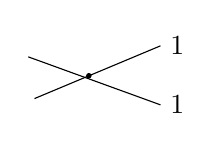
\begin{tikzpicture}[x=1cm,y=1cm]
\draw (0,0.05)--(1.6,.72) node[right] {$1$};
\draw (-.08,.58)--(1.6,-.03) node[right] {$1$};
\fill (.69,.34) circle (.035);
\end{tikzpicture}}
\[
f\omega=\varpi\qquad \omega=\frac{\varpi}{f}\qquad \widehat\omega=\frac{df}{f}
\]
\[
\operatorname{res}_{x}\omega\qquad \omega_i-\frac{df}{f}\qquad
\omega_i-\frac{df}{f}\quad\text{holomorphe au voisinage de}
\]
\[
\underline{\operatorname{Div}}_{X/S}\overset{\unsure{d\log f|d\log/S}}{\hookrightarrow}\underline R_{X/S}(\underline\Omega^1_{X/S})/\underline\Omega^1_{X/S}
\]
% The initial stroke curves upward at the left of the shaft.
% archive sheet number: 87
\scanpage{180}
$X$ \deleted{plat} au dessus de $S$

$Y$ sous-schéma divisoriel de $X$ transversal aux fibres est défini par un \uline{faisceau inversible} $\underline L$ sur $X$ et une section $s$ de $\underline L$ \deleted{\unsure{transv.}} non div de $0$ sur les fibres

Partons d'un faisceau inversible $\underline L$ sur $X$, et déterminons les \deleted{\unsure{faisc|faisceaux}} sous-schémas divisoriels $Y$ de $X$ transversaux aux fibres qui définissent des $\underline L(Y)$ \deleted{\unsure{iso}} qui sont \deleted{\unsure{Pic} $Y$-isomorphes}\deleted{\unsure{équivalents}} \deleted{à $\underline L$} isomorphes [resp\textsuperscript{t.} $\unsure{S|Y}$-équivalents, resp\textsuperscript{t.} \deleted{$Y$-équivalents} Pic\deleted{\unsure{$X/S$}}-équivalents rel. à $Y$] à $\underline L$. // Les premiers sont ceux qui se définissent par des sections de $\underline L$ non diviseurs de $0$ sur les fibres, sections qu'il faut prendre mod $\Gamma(S,f_*(\underline O_X^*))$ ; si $f_*(\underline O_X)=\underline O_S$, on les prend donc mod $\underline O_S^*$, donc on trouve les \unsure{quotients|partie} \deleted{de $\underline H_f^0(\underline L$} d'une \inserted{certaine} partie $\underline H^0_f(\underline L)^*$ de $\underline H_f^0(\underline L)$ par le groupe $\underline H^0_f(\underline O_X^*)=\unsure{\underline H_f^0|\underline W_f^0}(\underline O_X)^*$, donc dans le cas favorable par $\underline O_S^*$. --- Dans le deuxième cas, on trouve les \deleted{\unsure{éléments}}\inserted{sections} de $\underline H^0_f(\underline L)^*/\underline H_f^0(\underline O_X)^*$ donc dans le cas favorable de $\underline H^0_f(\underline L)^*/\underline O_S^*$. ---
% archive sheet number: 179
\scanpage{181}
Il en est encore de \unsure{$\overline{\mathrm m}$|même} pour le troisième, si on suppose que $X$ est \unsure{qu.|quasi} cpct séparé sur $S$ et que $\underline H_f^0(\underline O_X)=\underline O_S$ --- de sorte que la $S$-équivalence est identique à la Picard-équivalence rel. à $Y$

Supposons dorénavant que

$X$ qu-compact séparé sur $S$, $\underline H_f^0(\underline O_X)=\underline O_S$ et Kif kif par extension de la base

et que $\underline{\underline{\operatorname{Pic}}}_{X/S}$ et $\underline{\underline{\operatorname{Div}}}_{X/S}$ existent.

Alors l'ensemble précédent
\[
H^0(S,\underline H_f^0(\underline L)^*/\underline O_S^*)
\]
peut s'interpréter comme l'ensemble des sections $\theta$ de $\underline{\underline{\operatorname{Div}}}$ sur $S$ telles que
\diagram{\begin{tikzcd}[ampersand replacement=\&,column sep=small,row sep=small]
\underline{\underline{\operatorname{Pic}}}\arrow[dr,"\varphi"']\&\&\underline{\underline{\operatorname{Div}}}\arrow[ll,"p"']\arrow[dl,"\psi"]\\
\&S\&
\end{tikzcd}}
$p\theta=\lambda$, où $\lambda$ est la section de $\underline{\underline{\operatorname{Pic}}}$ sur $S$ qui correspond à $\underline L$. Donc, posons $\underline{\underline{\operatorname{Div}}}^{(L)}=\varphi^{-1}(\lambda(S))$ [sous-\unsure{préschéma} de $\underline{\underline{\operatorname{Div}}}$) c'est l'ens des sections de $\underline{\underline{\operatorname{Div}}}_{X/S}^{L}$ sur $S$. \deleted{\unsure{Donc}} Ceci est compatible avec extension de la base $S'$, donc le foncteur $\underline{\underline{\operatorname{Div}}}_{X/S}^{L}(S')=H^0(S',\underline H_{f'}^0(\underline L')^*/\underline O_{S'}^*)$ en $S'$ est représentable. \deleted{Ceci doit} [On obtient donc une condition nécessaire intéressante, en termes de diviseurs, \unsure{pour|que} l'existence
% archive sheet number: 180
\scanpage{182}
d'un préschéma de Picard \ldots] \deleted{\unsure{Ceci montre}.}

Utilisant ce résultat, on voit que \uline{si} on peut trouver un faisceau \inserted{\uline{inv}} fondamental \deleted{\unsure{un} $\underline\Lambda$} $\underline\Lambda$ sur $\underline{\underline{\operatorname{Pic}}}\times_S X$ \deleted{Alors ce faisceau} [par exemple si $X/S$ a une section \ldots], alors \deleted{$\underline{\underline{\operatorname{Div}}}_{X/S}$ s'identifie à}
\[
\underline{\underline{\operatorname{Div}}}_{X/S}\simeq
\underline{\underline{\operatorname{Div}}}^{\underline\Lambda}_{\underline{\underline{\operatorname{Pic}}}_{X/S}\times_S X\,/\,\underline{\underline{\operatorname{Pic}}}_{X/S}}
\]

Cela prouve l'intérêt d'une étude directe, indépendamment de celle de $\underline{\underline{\operatorname{Pic}}}_{X/S}$, des foncteurs \inserted{de la forme} $\underline{\underline{\operatorname{Div}}}_{X/S}^{\underline L}$ et des \deleted{\unsure{leurs représentants|leurs représentant}} préschémas qui dans les cas favorables les représentent.

On va supposer maintenant que $X$ est propre \inserted{et plat} sur $S$, et que l'on a un isom fonctoriel :
\[
\underline H_f^0(\underline L\otimes_{\underline O_S}\underline M)=\underline{\operatorname{Hom}}_{O}(\underline E,\underline M)
\]
pour $\underline M$ \unsure{qu. coh.} sur $S$ [ce qui est vrai si $S$ est local, \unsure{ou|où|et} $X$ projectif sur $S$] \deleted{\unsure{$X$ quasi libre sur $S$} \ldots]}.

La connaissance du faisceau cohérent $\underline E$ sur $S$ \deleted{fixe}\inserted{détermine} le ``foncteur'' $S'\rightsquigarrow\underline H^0_{f'}(\underline L')$. \uline{Supposons p. ex.} que
% archive sheet number: 181
\scanpage{183}
les fibres \unsure{de} $X/S$ soient \unsure{abs.|art.|rel.} \deleted{intègres}\inserted{primaires}. Alors on voit que l'on a

\margin{\uline{Prop}}
\[
\underline{\underline{\unsure{\operatorname{Dix}|\operatorname{Div}}}}_{X/S}^{\underline L}\simeq\underline P(\underline E)
\]
\uline{fibré projectif associé à} $\underline E$. Comme ce dernier est aussi isomorphe à $\operatorname{Proj}(\deleted{\unsure{\bigoplus|\underline E}}{\textstyle\coprod}_n\operatorname{Sym}^{n}(\underline E))$, \unsure{et|est} à fibres simples, on voit ceci :

\uline{Prop} Supposons $X/S$ \uline{primaire}. Alors \deleted{$\underline{\underline{\operatorname{Dix}}}^{L}_{X/S}$ est} les conditions suivantes sont équivalentes :

(i) $\underline{\underline{\operatorname{Div}}}_{X/S}^{L}$ est plat sur $S$ en $s$

% slanted
\margin{\deleted{\unsure{Doit}} \unsure{Dégager dès|Diagramme dès} $\hookrightarrow$ \unsure{que le mm sur} les fibrés projectifs}
(ii) $\underline{\underline{\operatorname{Div}}}_{X/S}^{L}$ est \uuline{simple} sur $S$ en $s$

(iii) Pour $n$ grand, $\operatorname{Sym}^{n}(\underline E)$ est loc libre sur $S$ en $s$

(iv) Pour \inserted{$k$ convenable,} $n$ grand, $\operatorname{Sym}^{nk}(\underline E)$ est loc. libre sur $S$ \inserted{en $s$} pour tt $n$ grand.

\diagram{\begin{tikzcd}[ampersand replacement=\&,row sep=tiny]
{\text{(i)}}\arrow[dd,Rightarrow,bend right=22]\\
{\text{(ii)}}\arrow[u,Rightarrow]\\
{\text{(iii)}}\arrow[d,Rightarrow]\\
{\text{(iv)}}\arrow[uuu,Rightarrow,bend left=44]
\end{tikzcd}}
(v) $\underline E$ est \deleted{libre} loc libre sur $S$ en $s$

\margin{par déf. $\unsure{\Updownarrow}$}
(vi) $\underline L$ est \unsure{co-plat|$0$-plat} rel. $S$

\margin{par Künneth}
(vii) $\underline H_f^0(\underline L)_{\inserted{s}}\deleted{\unsure{\otimes|\otimes k(s)}}\longrightarrow H^0(X_s,\underline L_{(s)})$ est \uuline{surjectif}
% archive sheet number: 182
\scanpage{184}
\unsure{Groupes|Groupe} de Picard des cônes et \unsure{de|des} leurs anneaux locaux au sommet
% archive sheet number: 183
\scanpage{185}
\uline{Groupe de Picard des cones} \uline{\unsure{épointés|épointis}}

$X\subset P_k^{r}$, cône projetant (affine) $C$, $a$ l'\deleted{origine} sommet, $C_a=\operatorname{Spec}\underline O_{C,a}$.

$C-a$ est un fibré principal sur $X$, de groupe $G_m$, dont la classe est celle $\xi\in\operatorname{Pic}(X)$ de $\underline O_X(1)$. Donc \uline{si} $X$ \uline{est régulier}
\[
\operatorname{Pic}(C-a)\xleftarrow{\sim}\operatorname{Pic}(X)/\mathbb Z.\xi
\]

Considérons le morphisme naturel
\[
C_a-a\longrightarrow C-a,
\]
il induit un hom canonique
\diagram{\begin{tikzcd}[ampersand replacement=\&,row sep=tiny]
\operatorname{Pic}(C-a)\arrow[r]\&\operatorname{Pic}(C_a-a)\\
\&{\displaystyle\lim_{U\ni a}\operatorname{Pic}(U-\unsure{a})}\arrow[u,phantom,"\rotatebox{90}{$\simeq$}" description]
\end{tikzcd}}

Je dis que c'\uline{est un isomorphisme si $X$ est régulier}. Comme pour $U=C-Y$ voisinage de $a$, on a
\[
\operatorname{Pic}(U-a)\simeq\operatorname{Pic}(C-a)/\operatorname{Im}\mathbb Z^{(I)}
\]
où $I$ est l'ens des comp. irréd. de $Y$,
% archive sheet number: 184
\scanpage{186}
l'assertion précédente équivaut à celle-ci :

\uline{pour tout diviseur} $D$ \uline{sur} $C$ \uline{tel que} $a\notin\operatorname{supp}D$, \uline{on a} $D\sim 0$ \uline{dans} $C-a$.

Pour le prouver, introduisons le cône projetant projectif $\widehat C$, et $E=\widehat C-a$, qui est un fibré vectoriel sur $X$ [savoir celui associé de façon covariante à $\underline O_X(1)$]. Alors $D$ provient d'un diviseur $\widehat D$ sur $\widehat C$ tel que $a\notin\operatorname{supp}\widehat D$, et par suite le \deleted{support de $\widehat D$ a} diviseur $\deleted{\unsure{E}}\unsure{D'|D}$ sur $E'$ induit par $\widehat D$ est \uline{à support propre} \uline{sur $X$}. Nous allons prouver le

\uline{Lemme} Soit $X$ préschéma régulier, $E$ un fibré vectoriel \inserted{de rang $1$} sur $X$ ($E=\underline W(\underline E)$, où $\underline E$ est un faisceau inv. sur $X$) $D$ un diviseur sur $E$, tel que suppt
% archive sheet number: 185
\scanpage{187}
soit propre sur $X$. \deleted{Alors} Soit $V=E-g(X)$, où $g$ est la section unité, alors
\[
D\cap V\sim0\quad\text{dans }V.
\]

\diagram{\begin{tikzcd}[ampersand replacement=\&]
E\arrow[d,"f"']\& E'\arrow[l,"h'"']\arrow[d,"f'"]\\
X\& X'\arrow[l,"h"]\arrow[u,bend right=36,"q"']
\end{tikzcd}}
On peut supposer que $D$ est un diviseur irréductible, défini par un sous-préschéma fermé $X'$ de $E$. \deleted{\unsure{Faisons}}

Supposons d'abord $X'$ \uline{régulier}, faisons le changement de base $h:X'\longrightarrow X$, alors $E'$ sur $X'$ est muni d'une section naturelle $q$ telle que $h'q=$ immersion can. de $X'$ dans $X$. On a donc \deleted{dans Pic}\inserted{(raisonnant sur Pic\ldots]}
% slanted
\margin{N.B. Cela a un sens car $h'$ et $q$ sont finis\ldots}
\[
D=(h'_{*}q)_*(1_{X'})=h'_*(q_*{\unsure{q}}.1_{X'})
\]
Il est bien connu d'ailleurs que
\[
q_*(1_{X'})=f'{}^*(\xi_{E'})
\]
où $\xi_{E'}=\operatorname{Pic}(X')$ est la classe can. de $E'/X'$. D'ailleurs $\xi_{E'}=h^*(\xi_E)$, d'où
\[
\begin{aligned}
q_*(1_{X'})&=\deleted{\unsure{h}}f'{}^*h^*(\xi_E)=h'{}^*f^*(\xi_E)\qquad\text{et}\\
\unsure{{}'D|D}&=h'_*h'{}^*(f^*(\xi_E))=f^*(\xi_E)\,h'_*(1_{E'})
\end{aligned}
\]
% archive sheet number: 186
\scanpage{188}
Or $h$ est un morphisme fini \inserted{de dim relative (\unsure{au sens|ou mieux} \unsure{cdr|cd|cds}) $0$}, soit $d$ son \deleted{\unsure{so}} degré, on a $h'_*(1^{\unsure{\cdot|'}})=d$ d'où
\[
D=d\,f^*(\xi_E)\quad -
\]
% slanted
\margin{Mérite de figurer dans le \unsure{livre}. Se généralise aux fibrés vectoriels de rang quelconque.}
Par suite
\[
D\cap V=d\bigl(f^*(\xi_E)\mid V\bigr)=\unsure{0}\quad-\qquad\text{cqfd.}
\]

Dans le cas général, supposant cependant le lieu singulier de $\deleted{\unsure{D}}X'$ fermé (plus gén, contenu ds un \deleted{\unsure{le}} fermé $\deleted{\unsure{Z'\subset}}Y'\subset X'$, $\ne X'$) on considère $Y=f(Y')$, et on applique ce qui précède à $X-Y$ et $D\mid X-Y$, et on gagne\ldots.

On trouve ainsi, dans le cas présent
\[
\boxed{\operatorname{Pic}(C-a)\simeq\operatorname{Pic}(C_a-a)\simeq\operatorname{Pic}(X)/\mathbb Z.\xi}
\]

Dans le cas où $C$ est normal (i.e. \deleted{\unsure{son}} $\underline O_{C,a}$ est normal) noter que $\operatorname{Pic}(C_a-a)$ est aussi le groupe $\operatorname{Cl}(\underline O_{C,a})$ des classes
% archive sheet number: 187
\scanpage{189}
de diviseurs de $\underline O_{C,c}$.

Posons
\[
\begin{aligned}
S&=\deleted{\operatorname{Spec}}C_a=\operatorname{Spec}\underline O_{C,a}\\
\widehat S&=\operatorname{Spec}\widehat{\underline O_{C,a}}
\end{aligned}
\]
nous avons un hom canonique
\[
\operatorname{Pic}(S-a)\longrightarrow\operatorname{Pic}(\widehat S-\hat a)
\]
[qui, dans le cas $S$ normal, s'interprète comme
\[
\operatorname{Cl}(S)\longrightarrow\operatorname{Cl}(\widehat S)\qquad ]
\]
et on peut se demander si c'est un isomorphisme. \deleted{Faisons écla} Pour ceci, nous allons interpréter l'hom précédent d'une autre manière. Soit $\widetilde C$ obtenu à partir de $C$ en ``faisant éclater l'origine'', donc $\widetilde C$ est un fibré vectoriel sur $X\simeq(\widetilde C)_a$, défini \deleted{\unsure{par des fibrés}} \inserted{comme $W(\underline O_X(-1))$}.

L'on a \deleted{$\unsure{\operatorname{Pic}(C_a-a}$}
\diagram{\begin{tikzcd}[ampersand replacement=\&]
\widetilde C\arrow[d]\&\widetilde C\times_{C_a}C=\widetilde S\arrow[l]\arrow[d]\\
C\&C_a=S\arrow[l]
\end{tikzcd}}
\diagram{\begin{tikzcd}[ampersand replacement=\&,column sep=small,row sep=small]
\operatorname{Pic}(C_a-a)\arrow[d,"\unsure{\sim|2|\wr}"]\&
\operatorname{Pic}(C-a)\arrow[l,"\sim"']\arrow[d,phantom,"\rotatebox{90}{$\simeq$}" description]\&
\deleted{\operatorname{Pic}(\widetilde C-X)}\arrow[l,"\deleted{\sim}"']\arrow[d,phantom,"\deleted{\simeq}" description]\\
\operatorname{Pic}(\widetilde S-X)\&\operatorname{Pic}(\widetilde C-X)\arrow[l,"\sim"']\&
\deleted{\operatorname{Pic}(\widetilde C)/\mathbb Z\,\unsure{p|D|\eta}}
\end{tikzcd}}
% archive sheet number: 188
\scanpage{190}
[N.B. $\operatorname{Pic}(\widetilde C-X)\simeq\operatorname{Pic}(\unsure{\bar C|\widetilde C})/\mathbb Z.\unsure{\eta|y}$, où où $\eta$ est la classe de $X$ considéré comme diviseur dans $\widetilde C$ ; \deleted{\unsure{$\xi$|et}} Comme $\operatorname{Pic}(\widetilde C)\xleftarrow{\sim}\operatorname{Pic}(X)$ par $\widetilde C\mathbin{-}X$, on retrouve ainsi l'isomorphisme $\operatorname{Pic}(C-a)\simeq\operatorname{Pic}(X)/\mathbb Z.\eta$].

D'autre part, on trouve aussi
\[
\operatorname{Pic}(\widehat S-\hat a)\simeq\operatorname{Pic}(\widetilde{\widehat S}-X)\simeq\operatorname{Pic}(\widetilde{\widehat S})/\mathbb Z\hat\eta
\]
où $\widetilde{\widehat S}$ désigne l'éclaté de $\widehat S$. Or on a un isom formel évident
\[
\widetilde{\widehat S}\simeq\widetilde S\times_S\widehat S\ \underset{\smash{\tikz[baseline=0pt]{\draw (0,.08)--(0,0)--(1.05,0)--(1.05,.08);}}}{\simeq\widehat{\widetilde S}}
\quad\text{(complété formel de $\widetilde S$ le long de $X$)}
\]
d'où, par le th. d'existence
\[
\operatorname{Pic}(\widetilde{\widehat S})\simeq\operatorname{Pic}(\widehat{\widetilde S})\ ;
\]
\deleted{comme par ailleurs} Ainsi, le \deleted{$\operatorname{Pic}(\widetilde{\widehat S}\unsure{-\hat a}$} morphisme
\[
\operatorname{Pic}(\deleted{\unsure{C_a}}S-a)\mathbin{-}\operatorname{Pic}(\widehat{\deleted{\unsure{C_a}}S}-a)
\]
est induit, en passant au quotient par $\mathbb Z\eta$ resp. $\mathbb Z\hat\eta$, par le morphisme
\[
\operatorname{Pic}(E)\longrightarrow\operatorname{Pic}(\widehat E)
\]
% archive sheet number: 189
\scanpage{191}
où $E$ est le fibré vectoriel $\widetilde C$ sur $X$, et $\widehat E$ son complété formel le long de $X$, donc
\[
\operatorname{Pic}(\widehat E)\simeq\deleted{\unsure{\operatorname{Pic}}}\varprojlim\operatorname{Pic}(E_n)
\]
où $E_n$ est le voisinage infinitésimal d'ordre $n$ de $X$ dans $E$,
\[
E_n=(X,\underline O_E/J^{n+1})
\]
$J$ étant l'idéal définissant $X$ dans $E$. Notons ici
\[
J/J^2=\underline O_X(1)
\]
\[
\operatorname{Pic}(E)\xleftarrow{\sim}\operatorname{Pic}(X)
\]
\inserted{Donc $\operatorname{Pic}(S-a)\mathbin{-}\operatorname{Pic}(\widehat S-\hat a)$ est inj (surj) sss $\operatorname{Pic}(E)\mathbin{-}\operatorname{Pic}(\widehat E)$ l'est.}

% slanted
On sait déjà \inserted{au moins dans le cas \deleted{\unsure{où}} $\unsure{\widehat S|S}$ normal\ldots.} \deleted{\unsure{que}} (et on voit immédiatement sur la dernière formule) que $\operatorname{Pic}(S-a)\mathbin{-}\operatorname{Pic}(\widehat S-\hat a)$ est \uline{injectif} donc $\operatorname{Pic}(E)\longrightarrow\operatorname{Pic}(\widehat E)$ est injectif [car $\operatorname{Pic}(X)\mathbin{-}\operatorname{Pic}(\widehat E)$ l'est, ayant l'inverse à gauche $\operatorname{Pic}(\widehat E)\mathbin{-}\operatorname{Pic}(E_0)=\operatorname{Pic}(X)$]

Reste à voir si $\operatorname{Pic}(E)\mathbin{-}\operatorname{Pic}(\widehat E)$ est bijectif. Grâce à $\operatorname{Pic}(X)\unsure{\simeq|\xrightarrow{\sim}}\operatorname{Pic}(E)$
% archive sheet number: 190
\scanpage{192}
\uline{il en est ainsi sss} $\operatorname{Pic}(\widehat E)\mathbin{-}\operatorname{Pic}(X)$ \uline{est injectif}, \deleted{\unsure{réciproque}}
\diagram{\begin{tikzcd}[ampersand replacement=\&,column sep=small]
\operatorname{Pic}(E)\arrow[r]\arrow[rr,bend right=22,"\sim"]\&
\operatorname{Pic}(\widehat E)\arrow[r]\&\operatorname{Pic}(X)
\end{tikzcd}}

Supposons p.ex que $\dim X=1$ ; alors \unsure{ds|dans} le système projectif $(\operatorname{Pic}(E_n))$, les morphismes de transition sont surjectifs. D'autre part, \inserted{en tous cas,} le noyau de $\operatorname{Pic}(E_n)\mathbin{-}\operatorname{Pic}(E_{n-1})$ $(n\geq1)$ est isomorphe à $H^1(X,J^n/J^{n+1})\simeq H^1(X,\underline O_X(n))$. Ainsi : \deleted{Si $X$ est de}

\uline{Proposition} Pour que $\operatorname{Pic}(E)\mathbin{-}\operatorname{Pic}(\widehat E)$ soit bijectif (ou encore $\operatorname{Pic}(S-a)\longrightarrow\operatorname{Pic}(\widehat S-\hat a)$ bijectif) il \deleted{faut} \uline{suffit} que l'on ait $H^1(X,\underline O_X(n))=0$ pour tt $n\geq1$ ; cette condition est aussi nécessaire si $\dim X=1$.

\unsure{Notons|Noter|Mais} que cette condition n'est \uline{pas remplie} si $d^\circ\underline O_X(1)<g-1$, $X$ étant lisse \unsure{irréductible} de genre $g$.

% slanted
\margin{\uline{Corollaire}\,\rule[-.8em]{.35pt}{2.3em}\hspace{.16em}\rule[-.8em]{.35pt}{2.3em}}
Mais soit $X$ \inserted{$\subset P_k^2$} une courbe plane lisse $/k$, de degré $d$, alors $g=1+\frac{d(d-3)}{2}$, et si $d<g-1$ i.e. $d\geq6$, \uline{cette condition n'est jamais remplie}
% archive sheet number: 191
